% Sum-product exponents for four families (generated by a script).
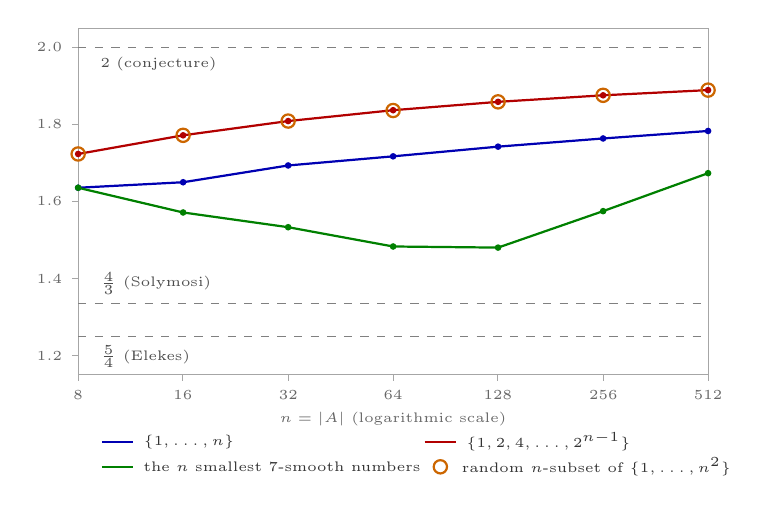
\begin{tikzpicture}[x=1cm,y=1cm]
\draw[black!35] (0,0) rectangle (8.00,4.40);
\draw[black!35] (0,0.24)--(-0.08,0.24) node[left,font=\tiny,black!60]{$1.2$};
\draw[black!35] (0,1.22)--(-0.08,1.22) node[left,font=\tiny,black!60]{$1.4$};
\draw[black!35] (0,2.20)--(-0.08,2.20) node[left,font=\tiny,black!60]{$1.6$};
\draw[black!35] (0,3.18)--(-0.08,3.18) node[left,font=\tiny,black!60]{$1.8$};
\draw[black!35] (0,4.16)--(-0.08,4.16) node[left,font=\tiny,black!60]{$2.0$};
\draw[black!35] (0.00,0)--(0.00,-0.08) node[below,font=\tiny,black!60]{$8$};
\draw[black!35] (1.33,0)--(1.33,-0.08) node[below,font=\tiny,black!60]{$16$};
\draw[black!35] (2.67,0)--(2.67,-0.08) node[below,font=\tiny,black!60]{$32$};
\draw[black!35] (4.00,0)--(4.00,-0.08) node[below,font=\tiny,black!60]{$64$};
\draw[black!35] (5.33,0)--(5.33,-0.08) node[below,font=\tiny,black!60]{$128$};
\draw[black!35] (6.67,0)--(6.67,-0.08) node[below,font=\tiny,black!60]{$256$};
\draw[black!35] (8.00,0)--(8.00,-0.08) node[below,font=\tiny,black!60]{$512$};
\node[below,font=\tiny,black!60] at (4.00,-0.35) {$n=|A|$ (logarithmic scale)};
\draw[black!50,dashed] (0,0.49)--(8.00,0.49) node[pos=0.02,below right,font=\tiny,black!70]{$\frac54$ (Elekes)};
\draw[black!50,dashed] (0,0.90)--(8.00,0.90) node[pos=0.02,above right,font=\tiny,black!70]{$\frac43$ (Solymosi)};
\draw[black!50,dashed] (0,4.16)--(8.00,4.16) node[pos=0.02,below right,font=\tiny,black!70]{$2$ (conjecture)};
\draw[blue!70!black,thick] (0.000,2.374) -- (1.333,2.444) -- (2.667,2.657) -- (4.000,2.773) -- (5.333,2.896) -- (6.667,3.000) -- (8.000,3.095);
\fill[blue!70!black] (0.000,2.374) circle (1.2pt);
\fill[blue!70!black] (1.333,2.444) circle (1.2pt);
\fill[blue!70!black] (2.667,2.657) circle (1.2pt);
\fill[blue!70!black] (4.000,2.773) circle (1.2pt);
\fill[blue!70!black] (5.333,2.896) circle (1.2pt);
\fill[blue!70!black] (6.667,3.000) circle (1.2pt);
\fill[blue!70!black] (8.000,3.095) circle (1.2pt);
\draw[red!70!black,thick] (0.000,2.803) -- (1.333,3.040) -- (2.667,3.221) -- (4.000,3.359) -- (5.333,3.465) -- (6.667,3.548) -- (8.000,3.614);
\fill[red!70!black] (0.000,2.803) circle (1.2pt);
\fill[red!70!black] (1.333,3.040) circle (1.2pt);
\fill[red!70!black] (2.667,3.221) circle (1.2pt);
\fill[red!70!black] (4.000,3.359) circle (1.2pt);
\fill[red!70!black] (5.333,3.465) circle (1.2pt);
\fill[red!70!black] (6.667,3.548) circle (1.2pt);
\fill[red!70!black] (8.000,3.614) circle (1.2pt);
\draw[green!50!black,thick] (0.000,2.374) -- (1.333,2.060) -- (2.667,1.873) -- (4.000,1.628) -- (5.333,1.614) -- (6.667,2.077) -- (8.000,2.559);
\fill[green!50!black] (0.000,2.374) circle (1.2pt);
\fill[green!50!black] (1.333,2.060) circle (1.2pt);
\fill[green!50!black] (2.667,1.873) circle (1.2pt);
\fill[green!50!black] (4.000,1.628) circle (1.2pt);
\fill[green!50!black] (5.333,1.614) circle (1.2pt);
\fill[green!50!black] (6.667,2.077) circle (1.2pt);
\fill[green!50!black] (8.000,2.559) circle (1.2pt);
\draw[orange!80!black,thick] (0.000,2.803) circle (2.4pt);
\draw[orange!80!black,thick] (1.333,3.040) circle (2.4pt);
\draw[orange!80!black,thick] (2.667,3.221) circle (2.4pt);
\draw[orange!80!black,thick] (4.000,3.355) circle (2.4pt);
\draw[orange!80!black,thick] (5.333,3.465) circle (2.4pt);
\draw[orange!80!black,thick] (6.667,3.548) circle (2.4pt);
\draw[orange!80!black,thick] (8.000,3.614) circle (2.4pt);
\draw[blue!70!black,thick] (0.30,-0.85)--(0.70,-0.85) node[right,font=\tiny,black!80]{$\{1,\dots,n\}$};
\draw[red!70!black,thick] (4.40,-0.85)--(4.80,-0.85) node[right,font=\tiny,black!80]{$\{1,2,4,\dots,2^{n-1}\}$};
\draw[green!50!black,thick] (0.30,-1.17)--(0.70,-1.17) node[right,font=\tiny,black!80]{the $n$ smallest $7$-smooth numbers};
\draw[orange!80!black,thick] (4.60,-1.17) circle (2.4pt) node[right=4pt,font=\tiny,black!80]{random $n$-subset of $\{1,\dots,n^2\}$};
\end{tikzpicture}
